\documentclass[10pt]{beamer}

\usetheme[progressbar=frametitle]{metropolis}
% font options
\usefonttheme{professionalfonts}
\usepackage{appendixnumberbeamer}

\usepackage{booktabs}
\usepackage[scale=2]{ccicons}

\usepackage{pgfplots}
\usepgfplotslibrary{dateplot}

\usepackage{lmodern}

\usepackage{cancel}

\usepackage{color}

\usepackage{xspace}
\usepackage{siunitx}
\newcommand{\themename}{\textbf{\textsc{metropolis}}\xspace}

\usepackage[usestackEOL]{stackengine}

\title{Mixed Hybrid Finite Element Eddington Acceleration of Discrete Ordinates Source Iteration}
\subtitle{\normalsize ANS Student Conference \\ Mathematics and Computation}
% \date{\today}
\date{April 10, 2017}
\author{Samuel S. Olivier}
\institute{Department of Nuclear Engineering, Texas A\&M University \\ \\ 
\scriptsize
% \url{https://github.com/smsolivier/EddingtonAcceleration.git} \\ 
\vfill
\centerline{
\includegraphics[height=.75cm]{nuen-logo.png}}}
% \titlegraphic{\hfill
\includegraphics[height=1.5cm]{nuen-logo.png}}

\newcommand{\SN}{S$_N$\xspace}
\renewcommand{\vec}[1]{\bm{#1}} %vector is bold italic
\newcommand{\vd}{\bm{\cdot}} % slightly bold vector dot
\newcommand{\grad}{\vec{\nabla}} % gradient
\newcommand{\ud}{\mathop{}\!\mathrm{d}} % upright derivative symbol
\newcommand{\pderiv}[2]{\frac{\partial #1}{\partial #2}}
\newcommand{\dderiv}[2]{\frac{\ud #1}{\ud #2}}
\newcommand{\edd}{\langle \mu^2 \rangle} 
\begin{document}

% make blocks fill 
\metroset{block=fill}

% dark background 
% \metroset{background=dark}

% color options
\definecolor{maroon}{RGB}{80,0,0}
\setbeamercolor{progress bar}{fg=maroon}
\setbeamercolor{progress bar in head/foot}{fg=maroon}
\setbeamercolor{progress bar in section page}{fg=maroon}

% \setbeamercolor{alerted text}{fg=maroon}

\maketitle

\begin{frame}{Overview}
  \setbeamertemplate{section in toc}[sections numbered]
  \tableofcontents[hideallsubsections]
\end{frame}

\section{Motivation}

% \begin{frame}{Radiation Hydrodynamics }
	
% 	Describes
% 	\vspace{-.05in}
% 	\begin{itemize}
% 		\item Propogation of thermal radiation through a fluid
% 		\item Effects of emission, absorption, scattering on fluid momentum and energy 
% 	\end{itemize}

% 	Required in high energy density laboratory physics (NIF, Z Machine) and astrophysics 

% 	Operator Split: advance hydrodynamics and radiation separately 

% 	Need hydrodynamics and transport to be consistently differenced  
% 	\vspace{-.05in}
% 	\begin{itemize}
% 		\item Use the same method or do extra work to make differing methods agree 
% 		\item Interpolating between spatial grids introduces noise 
% 		\item Matching grids between methods is not always possible in higher dimensions 
% 	\end{itemize}

% \end{frame}

\begin{frame}{Motivation}

	\footnotesize
	Radiation Hydrodynamics 
	\vspace{-.05in}
	\begin{itemize}
		\item Describes the effects of emission, absorption, scattering on fluid momentum and energy 
		\item Required in high energy density laboratory experiments (NIF, Z Machine) and astrophysics 
	\end{itemize}

	Mixed Hybrid Finite Element Method (MHFEM) hydrodynamics 

	Problems
	\vspace{-.05in}
		\begin{itemize}
			\item MHFEM and first-order form of transport are incompatible $\Rightarrow$ can't use linear acceleration scheme 
			\item Radiation transport is expensive 
		\end{itemize}

	\begin{block}{Goal}
		Develop a transport algorithm that 
			\begin{enumerate} \vspace{-.05in}
				\item \alert<2>{Accelerates Discrete Ordinates Source Iteration}
				\item Bridges Linear Discontinuous Galerkin (LDG) transport and MHFEM multiphysics
			\end{enumerate}
		\vspace{-.05in}
	\end{block}

\end{frame}

\section{Source Iteration Background}

\begin{frame}{Boltzmann Equation}
	Steady-state, mono-energetic, istropically-scattering, fixed-source \alert{Linear Boltzmann Equation} in 1D slab geometry:
	\begin{equation*}
		\mu \pderiv{\psi}{x}(x, \mu) + \Sigma_t(x) \psi(x,\mu) = 
		\frac{\Sigma_s(x)}{2} \int_{-1}^{1} \psi(x, \mu') d\mu' + \frac{Q(x)}{2}
	\end{equation*}

	$\mu = \cos \theta$ the cosine of the angle of flight $\theta$ relative to the $x$-axis

	$\Sigma_t(x)$, $\Sigma_s(x)$ total and scattering macroscopic cross sections 

	$Q(x)$ the isotropic fixed-source

	$\psi(x,\mu)$ the angular flux 

	% Factors of 1/2 come from 
	%     \begin{equation*}
	%         \phi(x) = \int_{-1}^{1} \psi(x,\mu) \ud \mu
	%     \end{equation*}

	\onslide<2>
	\vfill
	\centerline{\textbf{Integro-differential equation}}

\end{frame}

\begin{frame}{Discrete Ordinates (\SN) Angular Discretization}

	Compute angular flux on $N$ discrete angles
	\begin{equation*}
		\psi(x,\mu) \xrightarrow{\text{S}_N} 
		\begin{cases}
			\psi_1(x), & \mu = \mu_1 \\ 
			\psi_2(x), & \mu = \mu_2 \\ 
			\vdots \\ 
			\psi_N, & \mu = \mu_N 
		\end{cases}
	\end{equation*}

	\pause
	$\mu_1$, $\mu_2$, $\dots$, $\mu_N$ defined by $N$-point Gauss Quadrature Rule 

	\pause
	Integrate order $2N-1$ polynomials exactly with 
	\begin{equation*}
		\phi(x) = \int_{-1}^1 \psi(x, \mu) \ud\mu 
			\xrightarrow{\text{S}_N} \sum_{n=1}^N 
			w_n \psi_n(x)
	\end{equation*}

\end{frame}

\begin{frame}{\SN Equations}

	\begin{block}{\SN Equations}
	\begin{equation*}
		\mu_n \dderiv{\psi_n}{x}(x) + \Sigma_t(x) \psi_n(x) = 
		\frac{\Sigma_s(x)}{2} \phi(x) + \frac{Q(x)}{2} \,, \, 1 \leq n \leq N
	\end{equation*}
	\begin{equation*}
		\phi(x) = \sum_{n=1}^N w_n \psi_n(x)
	\end{equation*}
	\end{block}

	\textbf{$N$ coupled, ordinary differential equations}

	All coupling in scattering term 

\end{frame}

\begin{frame}{Source Iteration}

	Decouple by lagging scattering term 
	\begin{equation*}
		\mu_n \dderiv{\psi_n^{\ell+1}}{x}(x) + \Sigma_t(x) \psi_n^{\ell+1}(x) = 
		\frac{\Sigma_s(x)}{2} \phi^{\ell}(x) + \frac{Q(x)}{2} \,, 1 \leq n \leq N        
	\end{equation*}

	\textbf{$N$ independent, first-order, ordinary differential equations}

	Solve each equation with well-known sweeping process 

	\begin{exampleblock}{Source Iteration}
	\begin{enumerate}
		\item Given previous estimate for $\phi^{\ell}(x)$, solve for $\psi_n^{\ell+1}$

		\item Compute $\phi^{\ell+1}(x) = 
			\sum_{n=1}^N w_n \psi_n^{\ell+1}(x)$ 

		\item Update scattering term with $\phi^{\ell+1}(x)$ and repeat until: 
			 \begin{equation*}
				\frac{\|\phi^{\ell+1}(x) - \phi^{\ell}(x)\|}{\|\phi^{\ell+1}(x)\|} < \epsilon 
			 \end{equation*}

	\end{enumerate}
	\end{exampleblock}

\end{frame}

\begin{frame}{Need For Acceleration in Source Iteration}

	\onslide<1->
	Convergence rate is linked to the number of collisions in a particle's lifetime

	\onslide<2->
	If $\phi^0(x) = 0$
	\begin{equation*}
		\mu_n \dderiv{\psi_n^{1}}{x}(x) + \Sigma_t(x) \psi_n^{1}(x) =
		\vphantom{\cancelto{0}{\frac{\Sigma_s(x)}{2} \phi^{0}(x)}} 
		\cancelto{0}{\frac{\Sigma_s(x)}{2} \phi^{0}(x)}
		 + \frac{Q(x)}{2} \,, 1 \leq n \leq N 
	\end{equation*}
	\onslide<3->
	$\phi^1(x) $ is the uncollided flux 

	\onslide<4->
	$\phi^2(x)$ is uncollided and once collided flux 

	\onslide<5->
	\ $\vdots$

	$\phi^{\ell}(x)$ is the scalar flux of particles that have undergone at most $\ell - 1$ collisions 

	\onslide<6->
	\textbf{Slow to converge in optically thick systems with minimal losses to absorption and leakage}

\end{frame}

\begin{frame}{Need For Acceleration in Source Iteration}

	Radiation Hydrodynamics problems often contain highly diffusive regions 

	\SN is too expensive in these regions 

	Need an \alert{acceleration scheme} that rapidly increases the rate of convergence of source iteration 

\end{frame}

\section{Eddington Acceleration}

\begin{frame}{Conservative Form of Boltzmann Equation}

	% \pause
	% Boltzmann Equation
	% \begin{equation*}
	% 		\mu \dderiv{\psi}{x}(x, \mu) + 
	% 		\Sigma_t(x) \psi(x,\mu) = 
	% 		\frac{\Sigma_s(x)}{2} \phi(x) + 
	% 		\frac{Q(x)}{2} 
	% \end{equation*}

	Take moments of Boltzmann equation until have enough equations for the number of unknowns 

	\pause 
	Zeroth Moment: integrate over all angles \footnotesize
	\begin{equation*}
		\int_{-1}^{1} \mu \dderiv{\psi}{x}(x, \mu) \ud \mu \ + 
		\int_{-1}^{1} \Sigma_t(x) \psi(x,\mu) \ud \mu = 
		\int_{-1}^{1} \frac{\Sigma_s(x)}{2} \phi(x) \ud \mu \ + 
		\int_{-1}^{1} \frac{Q(x)}{2} \ud \mu 
	\end{equation*}
	\normalsize

	\pause
	Use $J(x) = \int_{-1}^{1} \mu \psi(x,\mu) \ud \mu$, 
		$\phi(x) = \int_{-1}^{1} \psi(x,\mu) \ud \mu$ 

	\pause
	\begin{block}{Zeroth Angular Moment}
	\begin{equation*}
		\dderiv{}{x} J(x) + \Sigma_a(x) \phi(x) = Q(x)
	\end{equation*}
	\end{block}

	\pause
	1 equation, 2 unknowns 

\end{frame}

\begin{frame}{Conservative Form of the Boltzmann Equation}

	First Moment: multiply by $\mu$ and integrate 
	{\footnotesize
	\begin{equation*}
		\only<1,2,3>{
		\int_{-1}^{1} \mu^2 \dderiv{\psi}{x}(x, \mu) \ud \mu}
		\only<4>{\alert{\int_{-1}^{1} \mu^2 \dderiv{\psi}{x}(x, \mu) \ud \mu}} \ + 
		\vphantom{\underbrace{\int_{-1}^{1} \mu \Sigma_t(x) \psi(x,\mu) \ud \mu}_{
			\Sigma_t(x) J(x)}}
		\only<1>{\int_{-1}^{1} \mu \Sigma_t(x) \psi(x,\mu) \ud \mu \ =}
		\only<2,3,4>{\underbrace{\int_{-1}^{1} \mu \Sigma_t(x) \psi(x,\mu) \ud \mu}_{
			\Sigma_t(x) J(x)
		} \ =}
		\only<1,2>{
		\int_{-1}^{1} \mu \frac{\Sigma_s(x)}{2} \phi(x) \ud \mu \ + \ 
		\int_{-1}^{1} \mu \frac{Q(x)}{2}  \ud \mu }
		\only<3,4>{\underbrace{
			\int_{-1}^{1} \mu \frac{\Sigma_s(x)}{2} \phi(x) \ud \mu + 
			\int_{-1}^{1} \mu \frac{Q(x)}{2}  \ud \mu 
		}_{\text{Isotropic} \Rightarrow 0}
		}
	\end{equation*}}

\end{frame}

\begin{frame}{Eddington Factor}

	Rearrange derivative 
	\only<1>{
	\begin{equation*}
		\dderiv{}{x} \int_{-1}^{1} 
			\mu^2 \psi(x,\mu) \ud \mu 
			\vphantom{
				\underbrace{
			\int_{-1}^{1} \mu^2 \psi(x,\mu) \ud \mu}_\text{Second Moment of $\psi$}
			}
	\end{equation*}
	}
	\only<2->{
	\begin{equation*}
		\dderiv{}{x} \underbrace{
			\int_{-1}^{1} \mu^2 \psi(x,\mu) \ud \mu}_\text{\tiny Second Moment of $\psi(x,\mu)$}
	\end{equation*}
	}

	\onslide<3->
	Each moment adds an equation and an unknown

	\onslide<4->
	Multiply and divide by $\int_{-1}^{1} \psi(x,\mu) \ud \mu$
	\begin{equation*}
		\only<4>{\dderiv{}{x} \int_{-1}^{1} \psi(x,\mu) \ud \mu \ }
		\only<5->{\dderiv{}{x} \underbrace{\int_{-1}^{1} \psi(x,\mu) \ud \mu
			\vphantom{
				\frac{
					\int_{-1}^{1} \mu^2 \psi(x,\mu) \ud \mu
				}{
					\int_{-1}^{1} \psi(x,\mu) \ud \mu
				}
			}}_{
			\phi(x)
		}}
		\only<4>{
			\frac{
				\int_{-1}^{1} \mu^2 \psi(x,\mu) \ud \mu
			}{
				\int_{-1}^{1} \psi(x,\mu) \ud \mu
			}
		}
		\only<5->{\underbrace{\frac{
			\int_{-1}^{1} \mu^2 \psi(x,\mu) \ud \mu
		}{
			\int_{-1}^{1} \psi(x,\mu) \ud \mu
		}
		}_{\edd(x)}
		}
		\vphantom{
			\underbrace{
			\frac{
				\int_{-1}^{1} \mu^2 \psi(x,\mu) \ud \mu
			}{
				\int_{-1}^{1} \psi(x,\mu) \ud \mu
			}
			}_{\edd(x)}
		}
	\end{equation*}

	\onslide<6->
	Eddington Factor 
	\begin{equation*}
		\edd(x) = \frac{\int_{-1}^1 \mu^2 \psi(x,\mu) \ud \mu}{
			\int_{-1}^1 \psi(x,\mu) \ud \mu
		}
	\end{equation*}

	\onslide<7->
	Angular flux weighted average of $\mu^2$

\end{frame}

\begin{frame}{Moment Equations}

	% \footnotesize
	\begin{block}{Moment Equations}
	\begin{equation*}
		\dderiv{}{x} J(x) + \Sigma_a(x) \phi(x) = Q(x) \tag{\footnotesize Zeroth Moment}
	\end{equation*}
	\begin{equation*}
		\dderiv{}{x} \edd(x) \phi(x) 
		+ \Sigma_t(x) J(x) = 0 
		\tag{\footnotesize First Moment}
	\end{equation*}
	\end{block}

	\pause 
	3 unknowns ($\phi(x)$, $J(x)$, $\edd(x)$), 2 equations 

	\pause 
	Closure: $\edd(x)$ found through Boltzmann Equation  

	\pause
	Moment Equations = angular flux informed diffusion

	\pause
	Transport information passed through $\edd(x)$ and boundary conditions

	% \pause
	% Just as accurate as \SN

	\pause 
	Analytically pointless: if Boltzmann can be solved, don't need Moment Equations 

	\pause 
	Numerically: use \SN to compute estimate of $\edd(x)$, Moment Equations to find $\phi(x)$

\end{frame}

\begin{frame}{Eddington Acceleration}

	\begin{exampleblock}{Eddington Acceleration}
	\begin{enumerate}
		\item Given the previous estimate for the scalar flux, $\phi^{\ell}(x)$, solve for $\psi_n^{\ell+1/2}(x)$

		\item \alert{Compute $\edd^{\ell+1/2}(x)$ }

		\item \alert{Solve the Moment Equations for $\phi^{\ell+1}(x)$ 
			using $\edd^{\ell+1/2}(x)$} 

		\item Update the scalar flux estimate with $\phi^{\ell+1}(x)$ and repeat the iteration process until the scalar flux converges
	\end{enumerate}
	\end{exampleblock}

	\pause
	Acceleration occurs because
	\begin{enumerate}
		\item Angular shape of the angular flux converges quickly $\Rightarrow$ Eddington factor quickly converges 

		\item Moment Equations model all scattering at once $\Rightarrow$ dependence on source iterations to introduce scattering information is reduced 

	\end{enumerate}

\end{frame}

\begin{frame}{Eddington Acceleration Properties}

	Produces 2 solutions (\SN and Moment)

	\pause
	Relaxes consistent differencing requirements important in linear acceleration 

	\pause 
	Transport can be LDG and Moment can be MHFEM 

	\pause 
	Moment Equations are conservative and relatively inexpensive to solve 

	\pause
	Downside: Which solution is correct? 

	\pause 
	Difference between \SN and Moment solutions can be used as a measure of mesh convergence 

\end{frame}

\section{Results}

% \begin{frame}{Test Problem} 

% 	Slab with reflecting left boundary and vacuum right boundary 

%     Thickness of \SI{20}{cm} 

%     $\Sigma_t(x) = \SI{1}{cm^{-1}}$

%     100 cells $\Rightarrow$ optical thickness of 20 and optical thickness per cell of 0.2 

%     S$_8$ solved with lumped Linear Discontinuous Galerkin 

%     Moment Equations solved with Mixed Hybrid Finite Element 

%     Compare to acceleration to constistently differenced S$_2$SA 

% \end{frame}

% \begin{frame}{Iterations to Convergence Comparison}

%     Vary ratio of $\Sigma_s$ to $\Sigma_t$ 

%     More scattering $\Rightarrow$ more diffusive, harder for \SN to solve 

%     \centerline{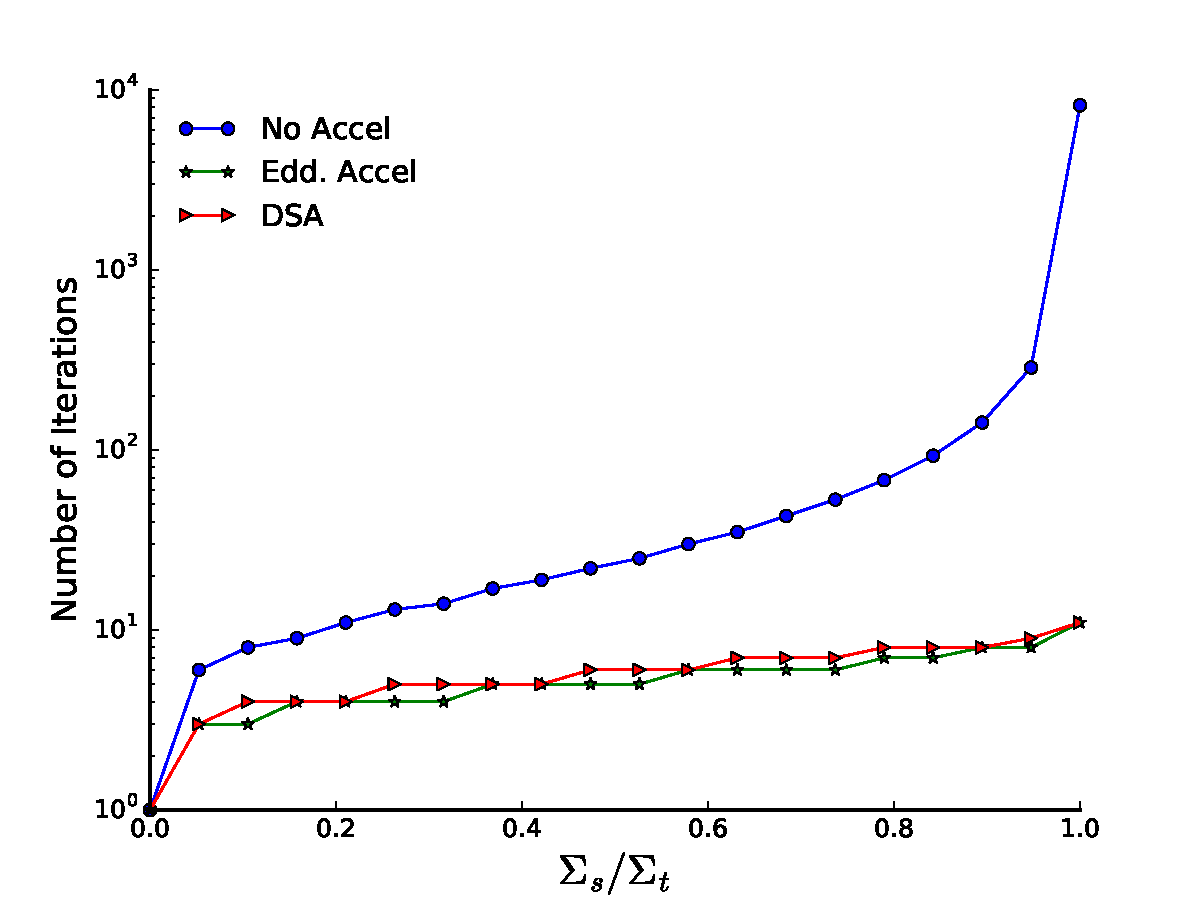
\includegraphics[width=.55\paperwidth]{figs/accel.pdf}}

%     Accelerates between 2.5 and 650 times $\Rightarrow$ acceleration is occurring 

%     Performs similarly to consistent acceleration scheme 

% \end{frame}

\begin{frame}{Test Problem}

	S$_8$ in 1D slab geometry 

	Lumped Linear Discontinuous Galerkin transport 

	Mixed Hybrid Finite Element Method Moment 

	\vfill
	\centerline{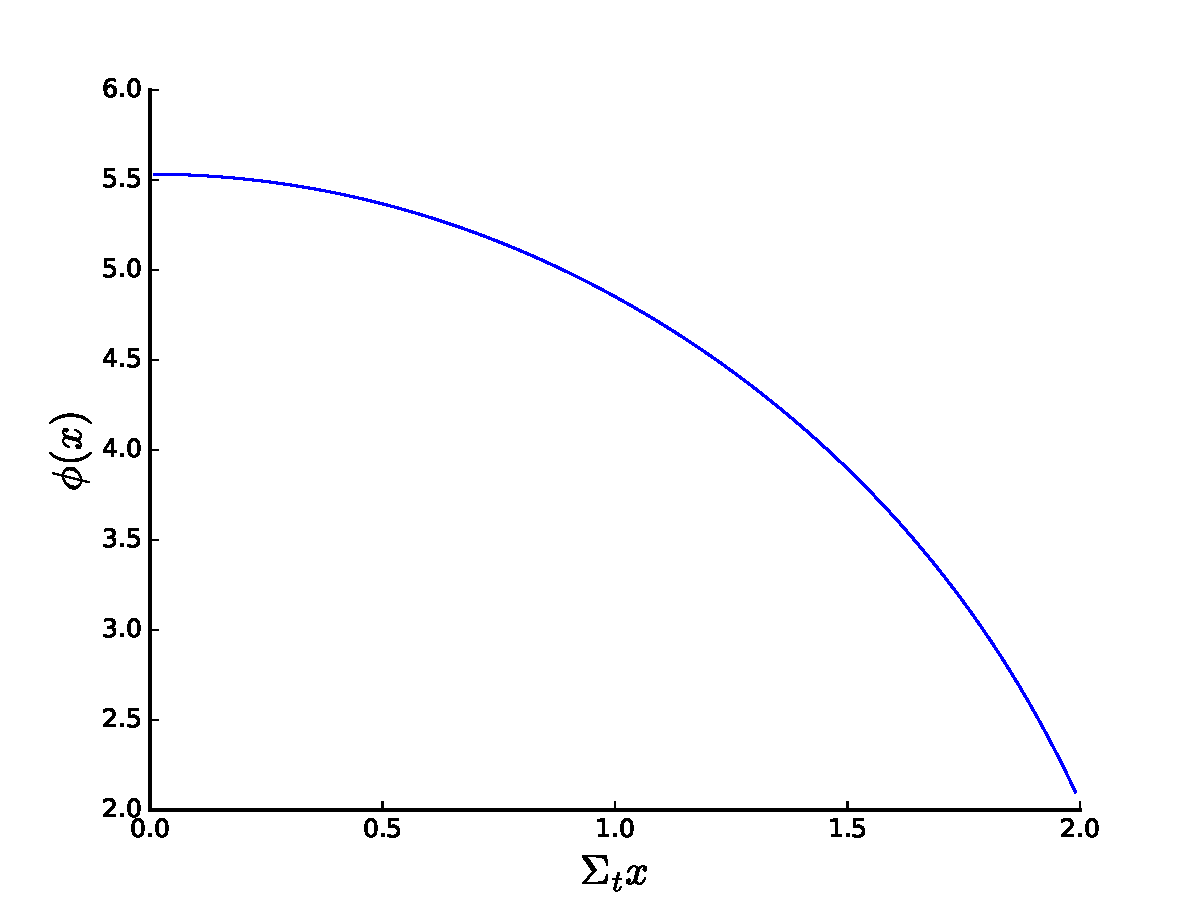
\includegraphics[width=.5\paperwidth]{figs/exSol.pdf}}

\end{frame}

\begin{frame}{Diffusion Limit}

	\footnotesize
	Scale cross sections, source 
	$$\Sigma_t \rightarrow \Sigma_t/\epsilon $$
	$$\Sigma_a \rightarrow \epsilon \Sigma_a$$
	$$Q \rightarrow \epsilon Q$$ 

	System becomes diffusive as $\epsilon \rightarrow 0$ 

	\pause
	\centerline{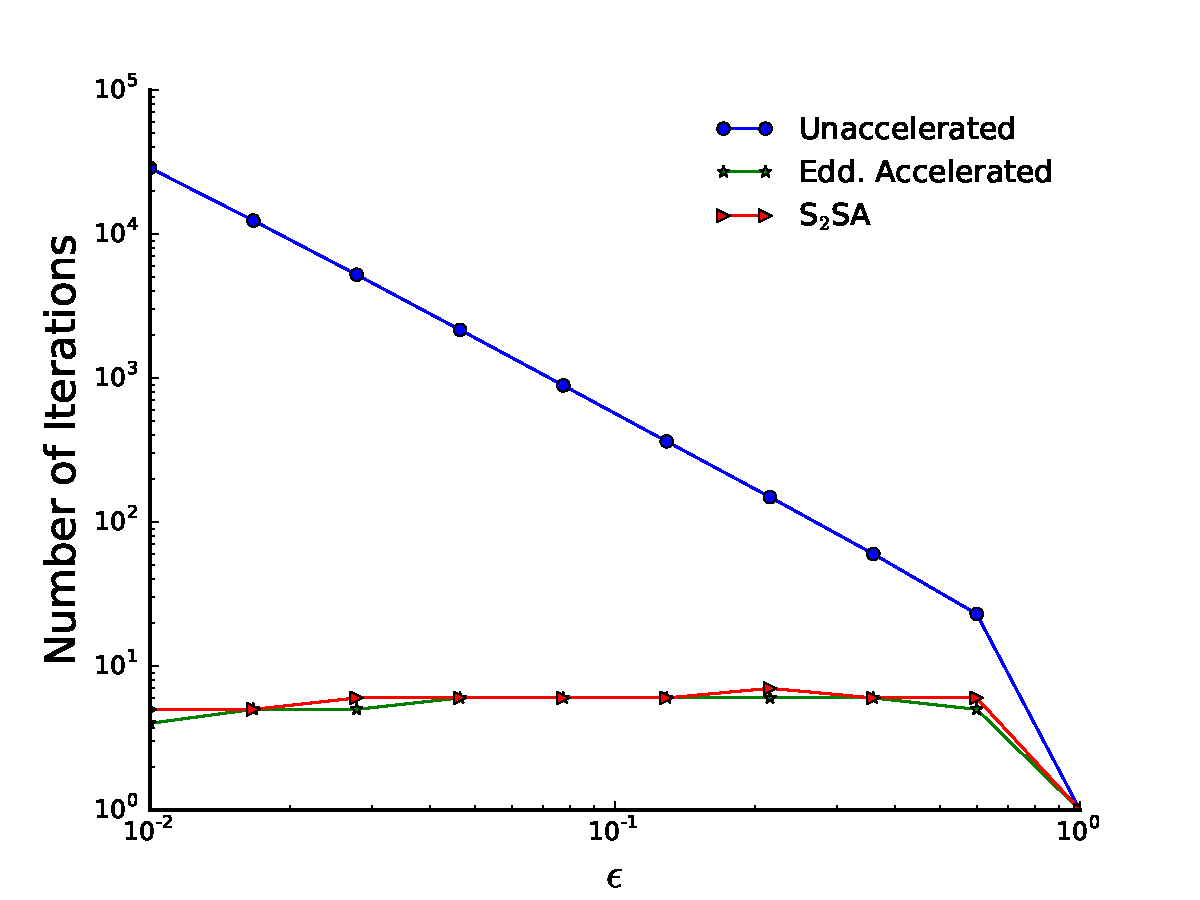
\includegraphics[width=.5\paperwidth]{figs/diffLimit.pdf}}

	\pause
	Survives diffusion limit 

	\pause
	Performs similarly to consistently differenced, linear acceleration (S$_2$SA)

\end{frame}

\begin{frame}{Convergence Rate Comparison}

	\begin{columns}
	\begin{column}{.5\paperwidth}
	\begin{figure} \centering
		Unaccelerated
		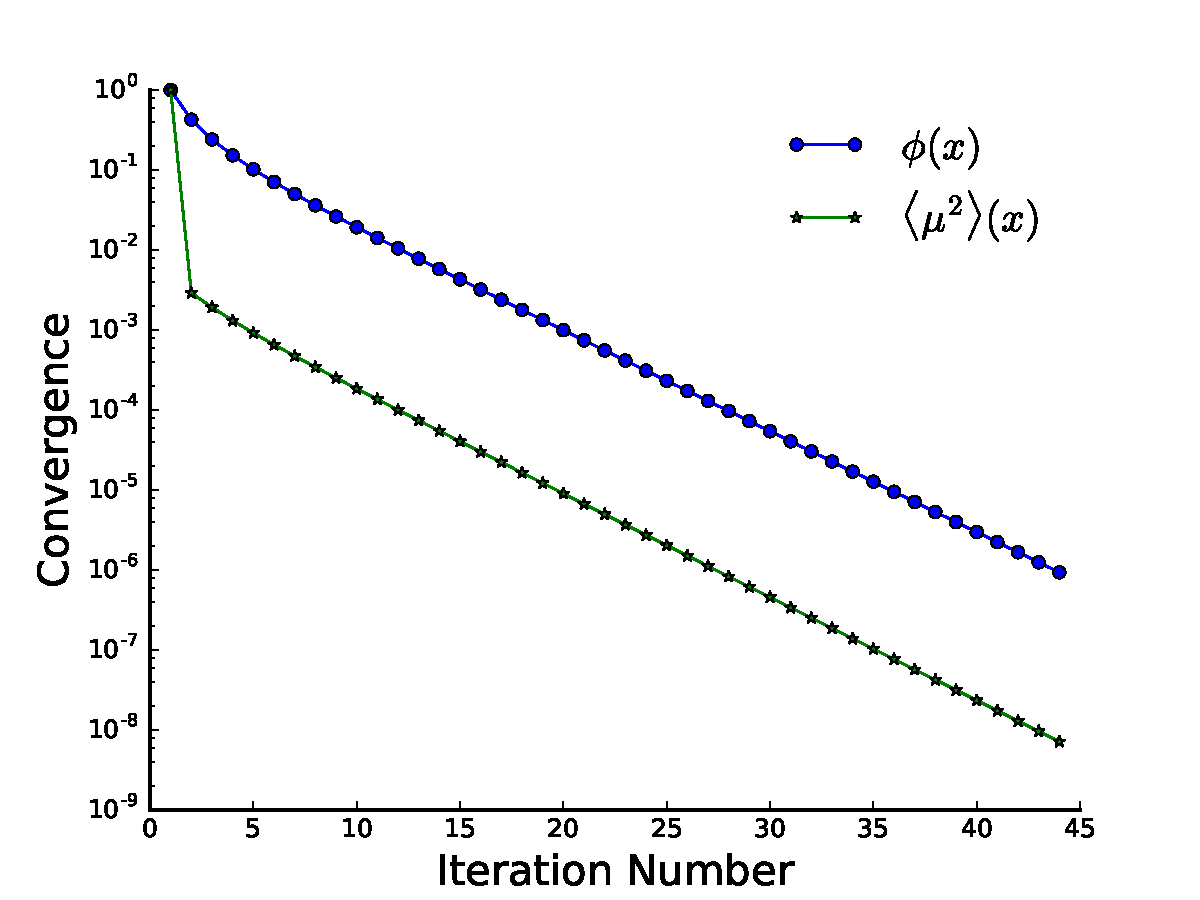
\includegraphics[width=.45\paperwidth]{figs/converge_una.pdf}
	\end{figure}
	\end{column}
	\pause
	\begin{column}{.5\paperwidth}
	\begin{figure} \centering
		Accelerated
		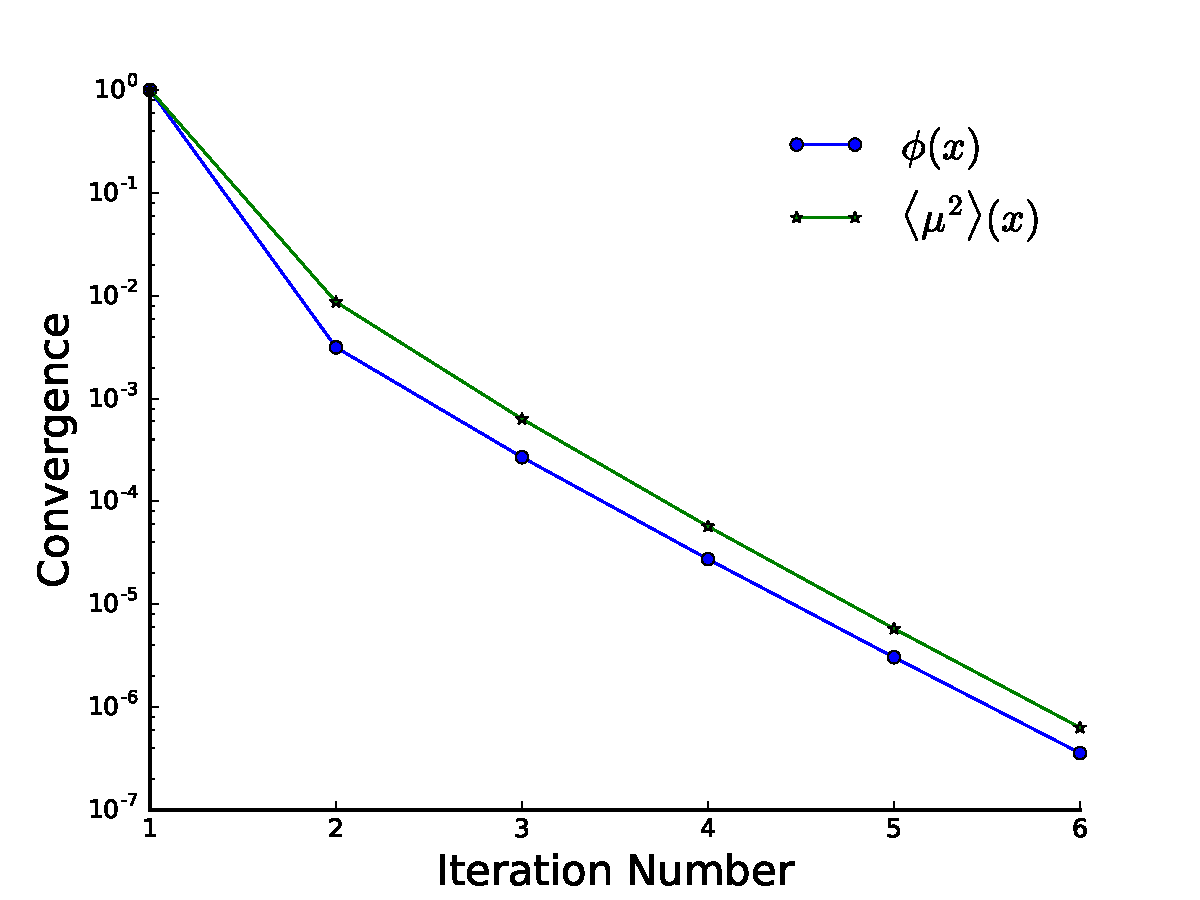
\includegraphics[width=.45\paperwidth]{figs/converge_acc.pdf}
	\end{figure}
	\end{column}
	\end{columns}

	\pause
	\vfill
	\centerline{\textbf{Fast rate of convergence of $\edd(x)$ is transfered to $\phi(x)$}}

\end{frame}

\begin{frame}{Method of Manufactured Solutions Order of Accuracy} 

	\footnotesize
	Set $Q(x)$ to force solution to 
	\begin{equation*}
		\phi(x) = \sin\left(\frac{\pi x}{x_b}\right)
	\end{equation*}

	Compare numerical results to MMS solution as cell width is decreased 

	\pause
	\centerline{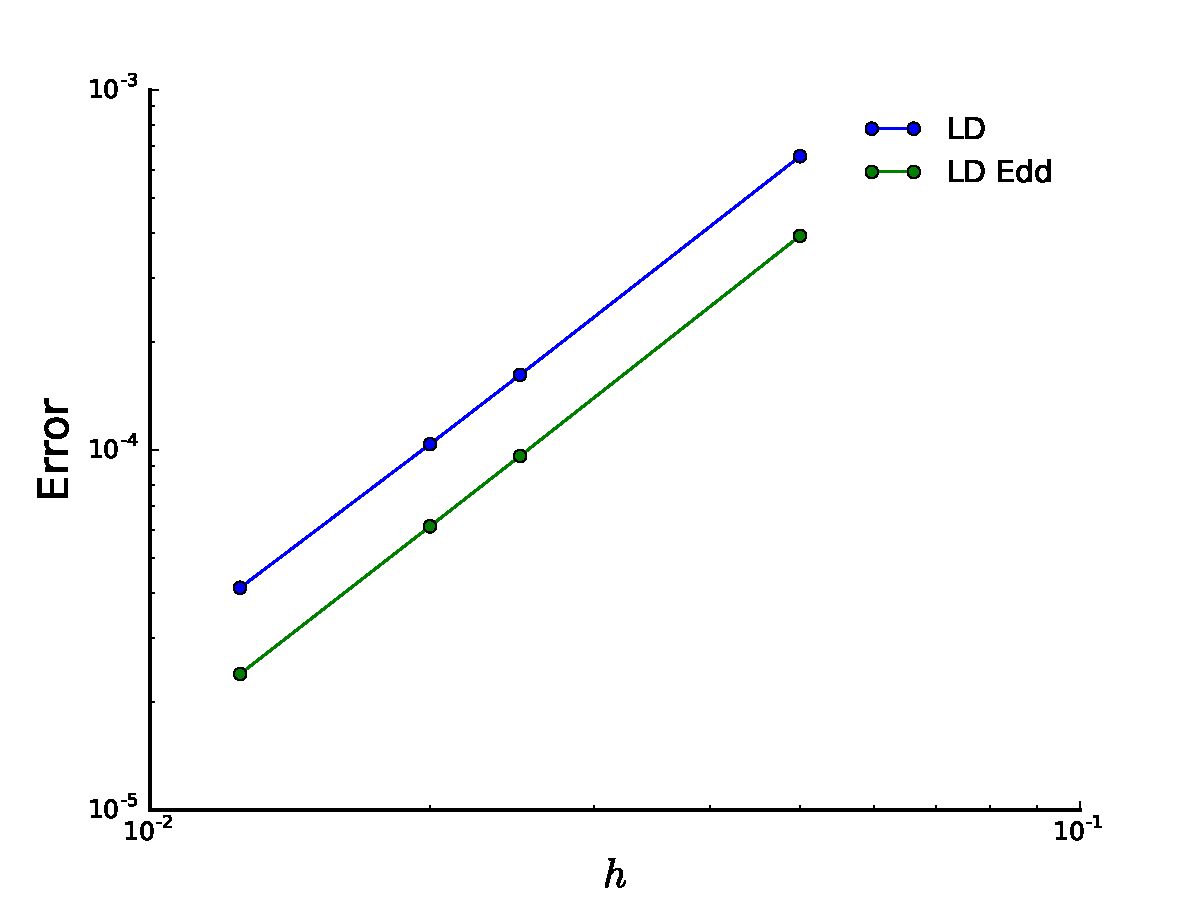
\includegraphics[width=.45\paperwidth]{figs/ooa.pdf}}

	\pause
	Data reconstruction: recover linear representation from MHFEM $\phi(x)$

	\pause 
	All second order as expected 

	\pause
	Eddington Acceleration did not effect the order of accuracy of lumped LDG 

	\pause 
	All slope recovery methods have similar accuracy 

\end{frame}

\begin{frame}{Data Reconstruction Solution Convergence}

	Compare 
	\begin{equation*}
		\frac{\| \phi_{\text{S}_N}(x) - 
			\phi_\text{Moment}(x)\|}{\|\phi_\text{Moment}(x) \|}
	\end{equation*}
	as $h\rightarrow 0$ 

	\pause
	\centerline{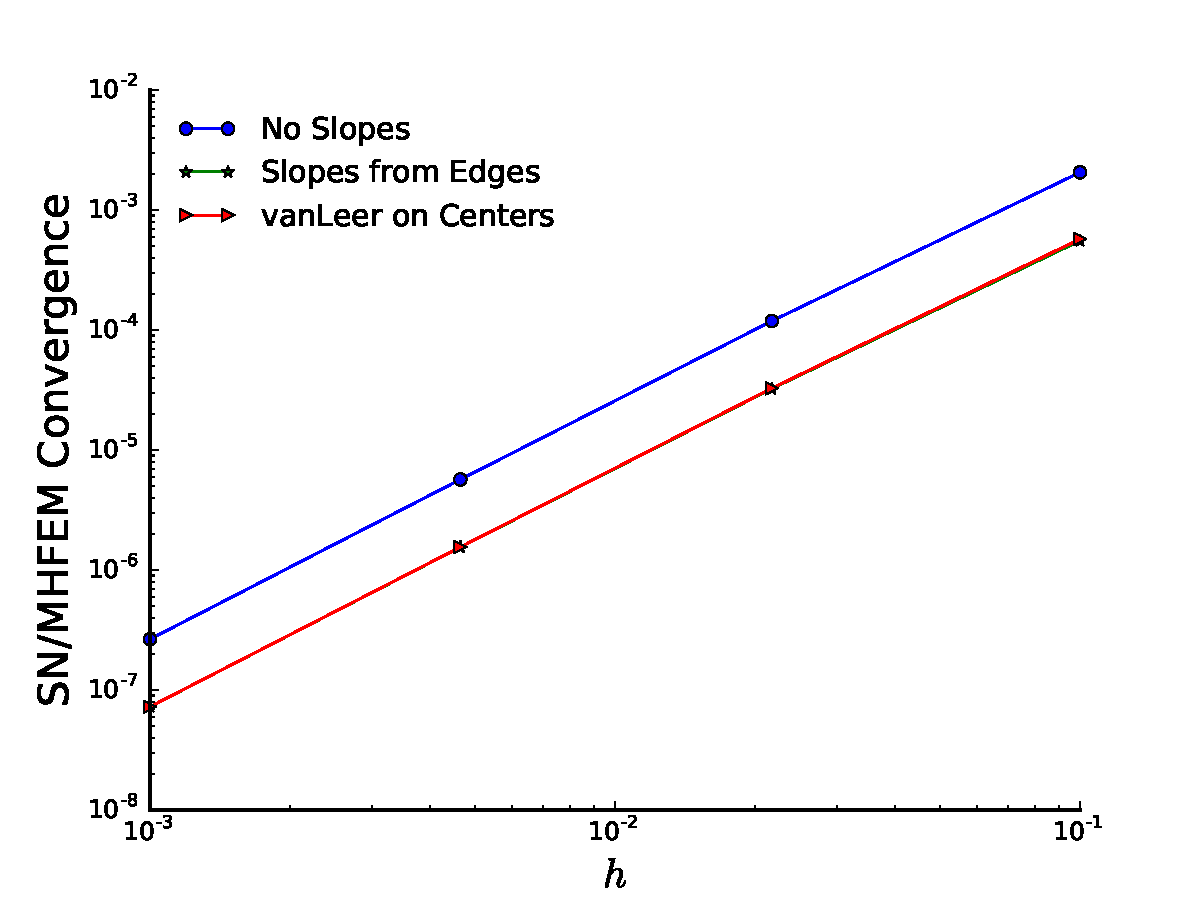
\includegraphics[width=.5\paperwidth]{figs/hlim.pdf}}

	\pause
	\SN and Moment solutions converge as mesh is refined 

	\pause Slope recovery effects solution convergence but not accuracy 

\end{frame}

\begin{frame}{Data Reconstruction Diffusion Limit}

	\centerline{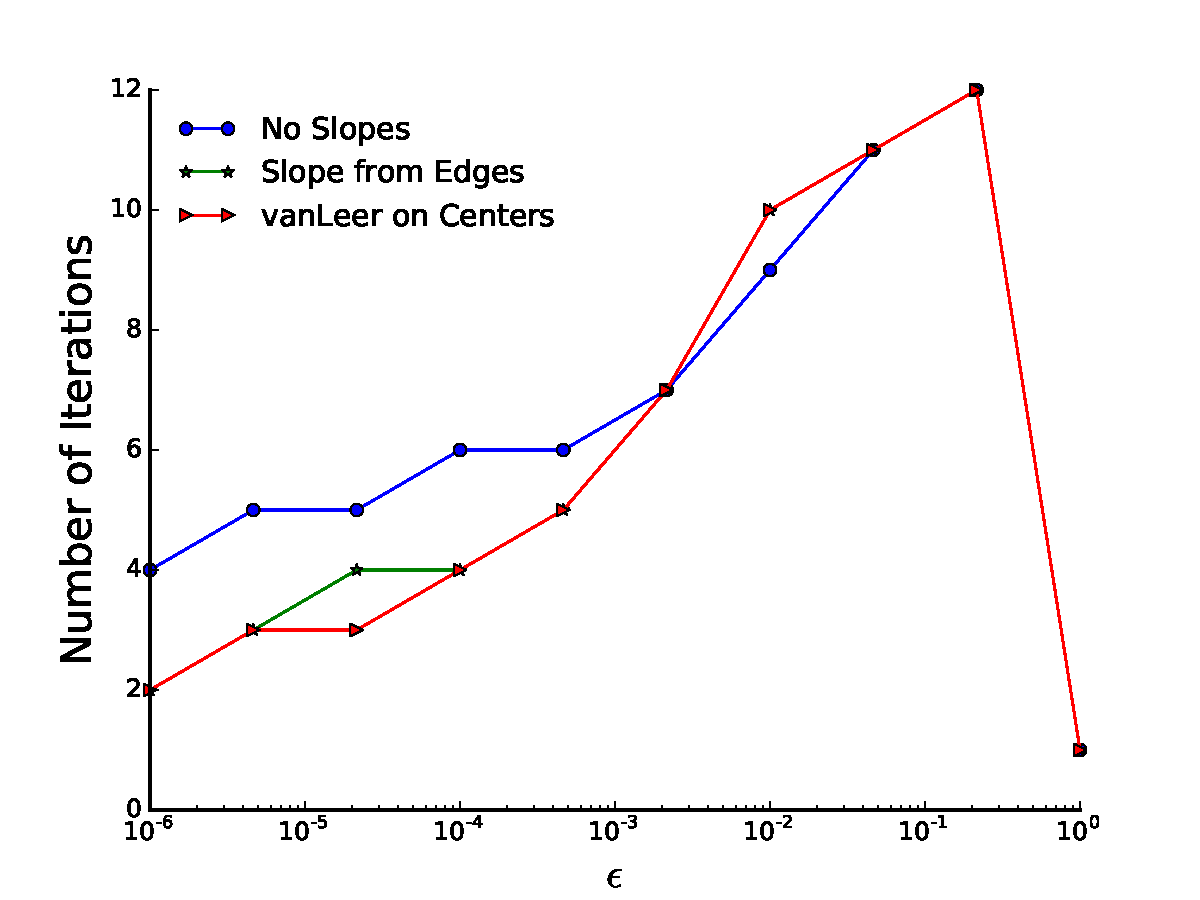
\includegraphics[width=.6\paperwidth]{figs/perm_dl.pdf}}

	\pause
	% \vfill
	All data reconstruction methods survived diffusion limit

	\pause
	\vfill
	\centerline{\textbf{Eddington Acceleration is extemely robust}}

\end{frame}

\section{Conclusions}

\begin{frame}{Summary}

	\onslide<+->
	Conclusions
	\begin{itemize} \vspace{-.1in}
		\item Scheme successfully accelerated source iteration in 1D slab geometry

		\item Eddington Acceleration is uniquely suited for radiation hydrodynamics 
		\begin{itemize}
			\item Transport and acceleration steps can be differenced with different methods 
			\item Reduces expense of source iteration 
			\item Provides inexpensive, conservative solution 
		\end{itemize}

		\item Showed MHFEM/LLDG pairing is robust 

	\end{itemize}

	\onslide<+->
	Future Work 
	\begin{itemize} \vspace{-.1in}

		\item Add temperature for radiative transfer 

		\item Higher dimensions 

		\item Develop an efficient rad hydro algorithm that makes use of the inexpensive Moment solution in multiphysics iterations 

	\end{itemize}

\end{frame}

% begin uncounted slides ---------------------------
\appendix

\begin{frame}{References}

	\nocite{adams,morel,llnl,alcouffe,mhfem,hydro,bolding,nonlinearAccel}
	\setbeamerfont{bibliography item}{size=\footnotesize}
	\setbeamerfont{bibliography entry author}{size=\footnotesize}
	\setbeamerfont{bibliography entry title}{size=\footnotesize}
	\setbeamerfont{bibliography entry location}{size=\footnotesize}
	\setbeamerfont{bibliography entry note}{size=\footnotesize}
	\setbeamertemplate{bibliography item}{\insertbiblabel}
	\bibliographystyle{siam}
	\bibliography{../bibliography}

\end{frame}

\begin{frame}[standout]
  Questions?
\end{frame}

\begin{frame}{Data Reconstruction Methods}

	MHFEM $\phi(x)$ is piecewise constant with discontinuous cell edges ($\phi_{i-1/2}$, $\phi_i$, $\phi_{i+1/2}$)

	LLDG is linear discontinuous ($\phi_{i,L}$, $\phi_{i,R}$)

	Need a way to recover slope information when \SN scattering term is updated with MHFEM $\phi(x)$ 

	No Slopes: 
	\begin{equation*}
		\phi_{i,L/R} = \phi_{i\mp1/2}^*
	\end{equation*}

	Slopes from Edges: 
	\begin{equation*}
		\phi_{i,L/R} = \phi_i^* \mp \frac{1}{2} \left(
		\phi_{i+1/2}^* - \phi_{i-1/2}^* \right)
	\end{equation*}

	vanLeer on Centers: 
	\begin{equation*}
		\phi_{i,L/R} = \phi_i^* \mp \frac{1}{4} \xi_\text{vanLeer} \left[ 
			\left(\phi_{i+1}^* - \phi_i^*\right) + \left(\phi_{i}^* - \phi_{i-1}^*\right)
		 \right]
	\end{equation*}

\end{frame}

\begin{frame}{S$_8$ v. Diffusion}

	Small system $\Rightarrow$ diffusion not expected to be accurate 
	\begin{center}
	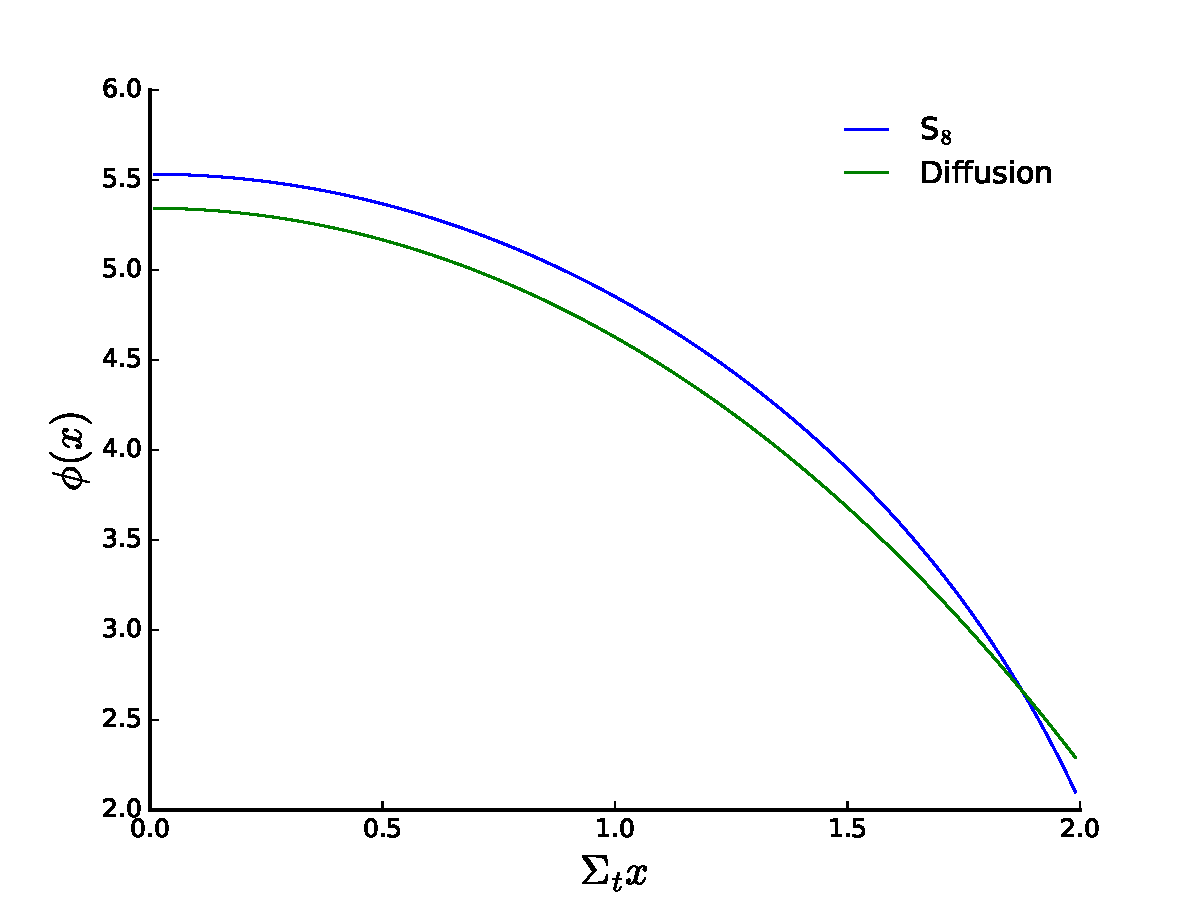
\includegraphics[width=.45\paperwidth]{figs/dvs.pdf}
	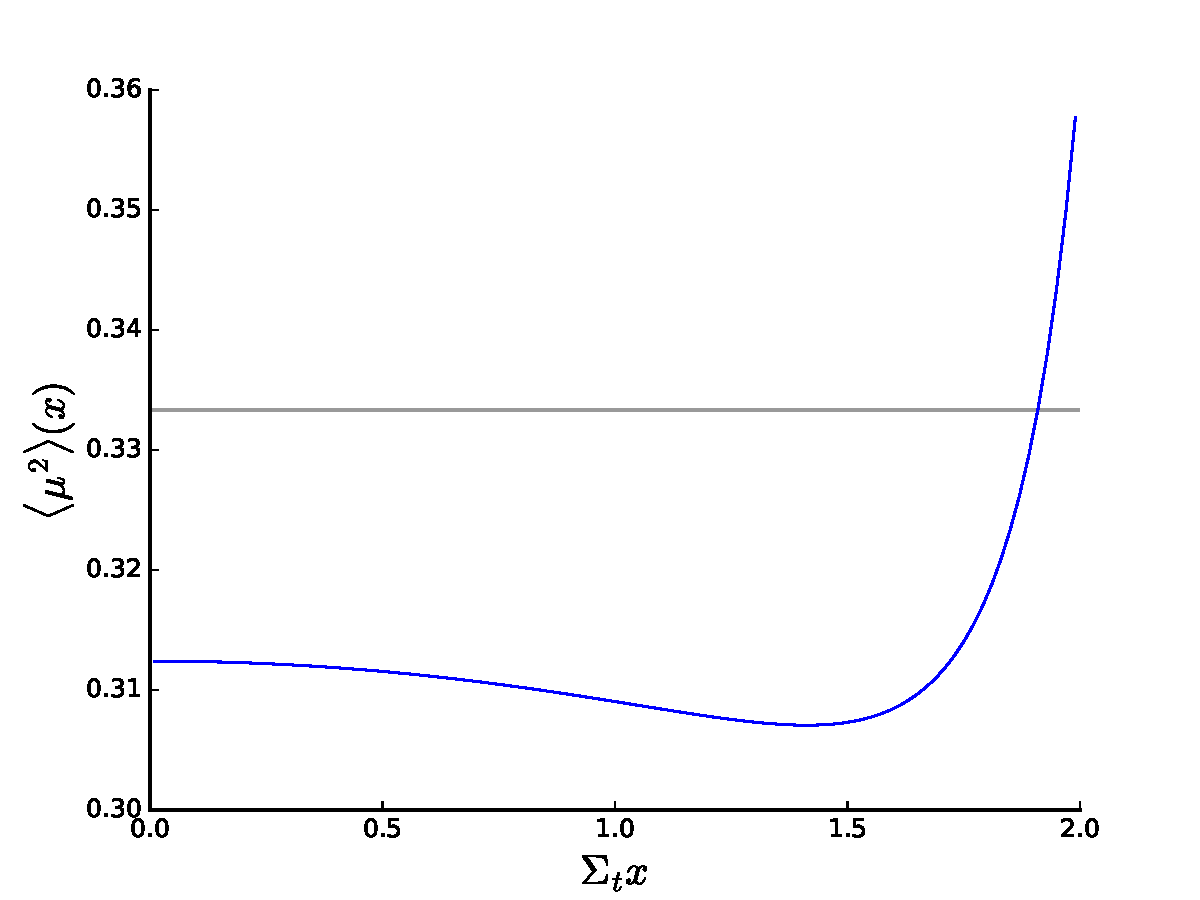
\includegraphics[width=.45\paperwidth]{figs/edd.pdf}
	\end{center}

\end{frame}

\begin{frame}{S$_8$ v. Drift Diffusion}

	\onslide<+->
	Use $\edd(x)$ from S$_8$ in Moment Equations
	\begin{center}
	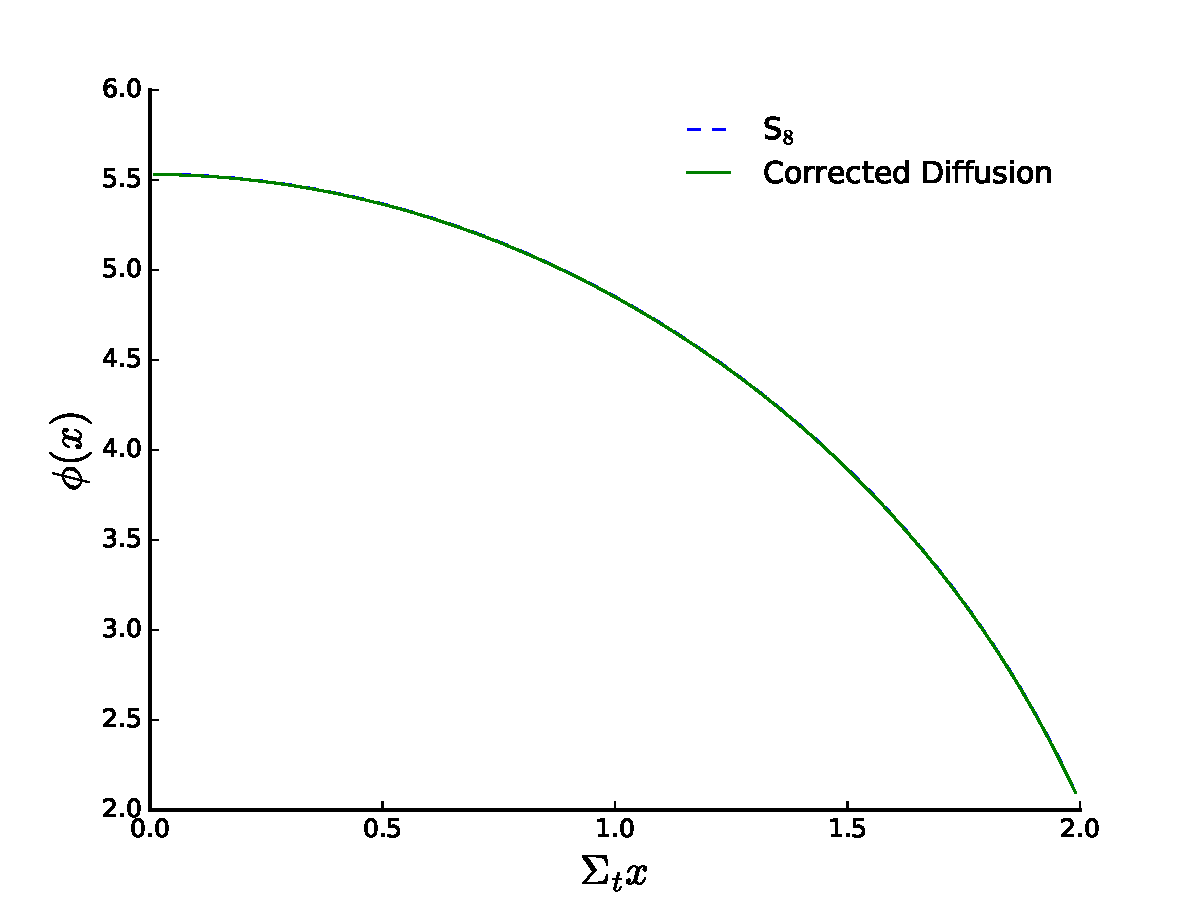
\includegraphics[width=.5\paperwidth]{figs/corrected.pdf}
	\end{center}

	\onslide<+->
	Moment Equations and \SN match! 

	\onslide<+-> 
	Requires knowledge of angular flux

\end{frame}

\end{document}
